%\documentclass[letterpaper, 10 pt, conference]{ieeeconf}  % Comment this line out
                                                         % if you need a4paper
\documentclass[a4paper, 10pt, conference]{ieeeconf}      % Use this line for a4
                                                         % paper

\IEEEoverridecommandlockouts                              % This command is only
                                                         % needed if you want to
                                                         % use the \thanks command
\overrideIEEEmargins
% See the \addtolength command later in the file to balance the column lengths
% on the last page of the document



% The following packages can be found on http:\\www.ctan.org
\usepackage{cite}
\usepackage[pdftex]{graphicx} % for pdf, bitmapped graphics files
%\usepackage{epsfig} % for postscript graphics files
%\usepackage{mathptmx} % assumes new font selection scheme installed
%\usepackage{times} % assumes new font selection scheme installed
\usepackage{amsmath} % assumes amsmath package installed
\usepackage{amssymb}  % assumes amsmath package installed
\newtheorem{theorem}{Theorem}

\title{\LARGE \bf Stochastic Strategies for a Swarm Robotic Assembly System}

%Chemical network modeling for top-down control design of an assembly
%task

%\author{ \parbox{3 in}{\centering Huibert Kwakernaak*
%         \thanks{*Use the $\backslash$thanks command to put information here}\\
%         Faculty of Electrical Engineering, Mathematics and Computer Science\\
%         University of Twente\\
%         7500 AE Enschede, The Netherlands\\
%         {\tt\small h.kwakernaak@autsubmit.com}}
%         \hspace*{ 0.5 in}
%         \parbox{3 in}{ \centering Pradeep Misra**
%         \thanks{**The footnote marks may be inserted manually}\\
%        Department of Electrical Engineering \\
%         Wright State University\\
%         Dayton, OH 45435, USA\\
%         {\tt\small pmisra@cs.wright.edu}}
%}

\author{Lo\"ic Matthey, Spring Berman and Vijay Kumar% <-this % stops a space
\thanks{}% <-this % stops a space
\thanks{
       {\tt\small }}%
\thanks{L. Matthey is with the DISAL Laboratory, Ecole Polytechnique Federale de Lausanne, Station 14, 1015 Lausanne, Switzerland,
{\tt\small loic.matthey@epfl.ch}}
\thanks{S. Berman and V. Kumar are with the GRASP Laboratory, University of Pennsylvania, 3330 Walnut Street, Philadelphia, PA 19104, USA,
       {\tt\small \{spring, kumar\}@grasp.upenn.edu}}
\thanks{We gratefully acknowledge partial support from NSF grants CSR-CPS
0720801, IIS-0427313, NSF IIP-0742304, and IIS-0413138, ARO grant
W911NF-05-1-0219, and ONR grant N00014-07-1-0829.} }


\begin{document}


\maketitle
\thispagestyle{empty}
\pagestyle{empty}


%%%%%%%%%%%%%%%%%%%%%%%%%%%%%%%%%%%%%%%%%%%%%%%%%%%%%%%%%%%%%%%%%%%%%%%%%%%%%%%%
\begin{abstract}


\end{abstract}


\section{INTRODUCTION}
   \section{Problem overview} % (fold)
\label{sec:problem_overview}

	Self-assembly is everywhere.
	
	\paragraph{}

	At every scale, systems interact, collaborate and combine to create new bigger scale systems. Crystals are formed by nanoscale assembly of carbon atoms, cell membranes by the arrangement of fatty acids into a lipid bilayer and human beings by the organization and cooperation of their trillions of living cells.

	Yet this process, being maybe so general and vast, is still tremendously unknown.

	The study of self-organizing systems gives insight into the organization patterns of their parts, and could help understanding and then modifying them.

	The recent field of Swarm intelligence applies the self-organizing principle to many systems and applications, ranging from algorithmic procedures (routing of packets, meta heuristics) to team of multiple robots. This approach makes sense when the number of robots increases to the point where a centralized or classical control methodology is not tractable anymore.
Interestingly, a similar problem occurs when the scale of robots and components starts to shrink down dramatically. If the environment is intrinsically random and unknown, the robustness factor promoted by self-organizing systems becomes a key factor.

	\paragraph{}
	Our interest goes towards that direction. We want to study systems whose dimension is shrinking to the level where classical approaches are not applicable anymore. Furthermore, we want to model those systems, and create a framework providing a complete control flow to modify the behavior of those systems.

	This might seem fairly trivial, but when the system under consideration is hard to study by definition and not well-known, even the simplest control over them or insight in their behavior becomes an appreciable achievement.

	\paragraph{}
	Our approach is the following:
	\begin{itemize}
		\item We propose an abstract way of describing the problem under study and the actions needed to achieve its control. Our main claim is that it is possible to divide the problem into two parts: an intrinsic system, on which we have no control, and an augmented system, which encompass our additions and modifications made to modify the behavior.
		\item We propose to use a Chemical Reaction Network mathematical framework through all this process to model the system under study. This framework will proves itself useful for its flexibility and expressive power at the scale we are studying.
		\item We present a way to control the system via a Top-down design approach, first working on the model and then mapping it back onto the studied system. Top-down design peaks the interest nowadays, as being able to control a complex system using high-level instructions only is a promising characteristic.
		\item Everything is presented and verified by referring to a specific system that we create and study: a robotic platform performing a self-assembly of products.
	\end{itemize}
	
	We call it the \textbf{Hybrid Reactions Modeling for Top-down Design Framework} (HyRToD). ``Hybrid'' because we will use both ordinary differential equations approximations and stochastic simulations to simulate the model, depending on the context.
	
	The robotic platform is actually simulated on a computer, by using a realistic 3D physics simulator named Webots~\cite{Michel:2004p10762}. Webots is based on ODE, an open source physics engine for simulating 3D rigid body dynamics~\cite{ode}. Such a simulator allows us to performs systematic experiments faster than real-time and with null fabrication costs.
	
	This might seems strange to apply a framework we claim to be thought for micrometer scale dynamics onto a high level robotic platform. We actually design the robotic platform to give it characteristics usually shown at a smaller scale, and therefore only take advantage of the robotic platform as a model system easy to measure and modify. This work focuses on this robotic platform as a first test for our framework. Further works will consider smaller scale applications to assess our initial assumption on our framework.
	
\subsection{Relations to biological processes} % (fold)
\label{sub:relations_to_biological_processes}
	Even though we apply our method to a robotic implementation, a fairly high scale system by all means, we claim that this method is applicable to many different systems, especially the ones governed by random dynamics.
	
	We chose to create a robotic platform performing a self-assembly task on purpose. Having robots carrying the building blocks and assembling them can be thought of as an idealization of the self-assembly process taking place into the cell, for example the protein synthesis. If we allow the building blocks to move around and assemble on their own, the added robots will behave like enzymes, promoting some reactions.
	
	Moreover, our method, using a Chemical Reaction Network model, is very easy to apply on biological processes. This model has been extensively used in the study of biological systems, and is very well understood by the community working in this field. This is an added factor to the development of further interdisciplinary cooperations between engineering and life sciences.
% subsection relations_to_biological_processes (end)


% section problem_overview (end)

\section{Outline} % (fold)
\label{sec:outline}
	This report is organized as follows: Chapter~\ref{cha:project_description} defines precisely our goals and the abstract problem definition and control flow we aim to study. Chapter~\ref{cha:field_overview} goes over the theoretical notions used in our work, and gives pointers to the available literature on the subject. Chapter~\ref{cha:puzzle_test_case_implementation} presents extensively the specific system we are studying, namely the physical robotic simulation of an assembly task. Chapter~\ref{cha:mathematical_model_of_the_puzzle_test_case} introduces the representation of our specific system into a Chemical Reaction Network notation, presents how we fitted the free parameters and compare the simulated results with the physical measurements. Chapter~\ref{cha:chemical_reaction_networks_control_and_design} is dedicated to the optimization step applied on our mathematical model in order to control its behavior. Chapter~\ref{cha:augmented_assembly_implementation} presents the Top-down mapping of the modified model towards the physical system. Chapter~\ref{cha:conclusion_and_outlook} concludes the work and assess its validity and shortcomings.
% section outline (end)

\section{PROBLEM STATEMENT}
   \subsection{Assembly task} % (fold)
\label{sub:assembly_task}

There are four different types of parts, numbered $1$ through $4$,
which can be combined to form larger parts according to the assembly
plans in Fig. \ref{fig:assembly_plans}. Parts bond together through
bi-directional connections at sites along their perimeters. The last
step in each plan is the production of a final assembly, $F1$ or
$F2$.  The assembly task is executed by a group of robots in an
arena that is sufficiently large to ignore the dynamics of
small-scale interactions.  Initially, robots and many copies of
parts of type $1$ through $4$ are randomly scattered throughout the
arena. There are exactly as many of these parts as are needed to
create a specified number of final assemblies, and the number of
robots equals the total number of scattered parts. Each robot knows
the assembly plans a-priori and has the ability to recognize part
types, pick up a part, combine it with one that is being carried by
another robot, and disassemble a part it is carrying.

Our objective is to define robot controllers for moving around the
arena and for picking up, assembling, and disassembling parts so
that the robots produce target numbers of final assemblies as
quickly as possible.

\begin{figure}[t]
    \centering
        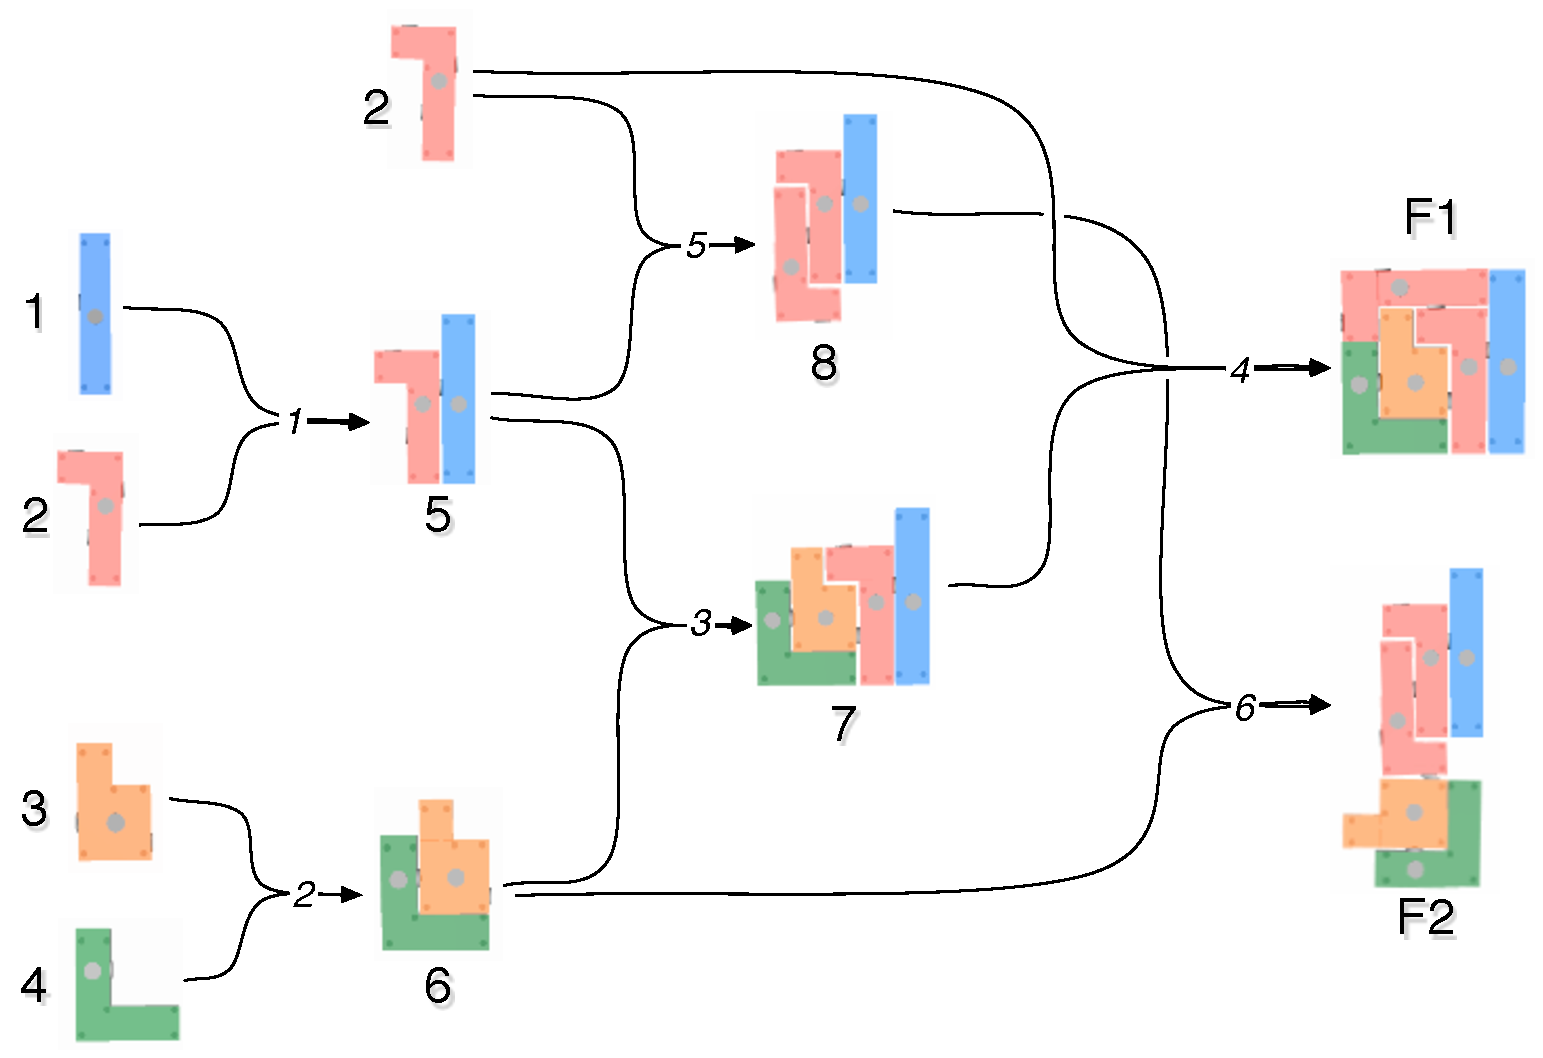
\includegraphics[width=8cm]{img/assembly_plans.pdf}
    \caption{Assembly plans for final assemblies F1 and F2.}
    \label{fig:assembly_plans}
\end{figure}


%, that can be combined into two possible final assemblies, $F1$ and
%$F2$.  Each final assembly is built from components $1, 3, 4$, and
%two copies of $2$ according to the plans in Fig.
%\ref{fig:assembly_plans}.

% subsection assembly_task (end)

\subsection{Micro-continuous model} % (fold)
\label{sub:stochastic_assembly}

We implement the assembly task in the robot simulator Webots
\cite{Michel:2004p10762}, which uses the Open Dynamics Engine to
accurately simulate physics.  We use the robot platform Khepera III,
which has infra-red distance sensors for collision avoidance. Each
robot is outfitted with a protruding bar with a rotational servo at
the tip.  A magnet on the servo bonds to a magnet on the top face of
a part, and the servo is used to rotate the bonded part into the
correct orientation for assembly.  Parts bond to each other via
magnets on their side faces.  Magnets can be turned off to
deactivate a bond.  Robots and parts are equipped with a radio
emitter and receiver for local communication and for computing
relative bearing, which is used to align robot and part magnets and
to rotate a part for assembly. The task takes place inside the
walled hexagonal arena shown in Fig. \ref{fig:overall_arena}.

We use a control policy for the robots that is inspired by chemical
processes: random movement patterns with probabilistic assemblies
upon encounter, as well as random disassemblies.  Our models assume
that the system is well-mixed; to achieve this property, robots move
according to a random walk, and we verify that the space is
uniformly covered. Robots and parts switch between action states
based on information they receive via local sensing and
communication.  When a robot encounters a part on the ground, it
approaches and bonds to it and starts searching for a robot that is
carrying a compatible part, according to the assembly plans.  When
one is found, the two robots align their parts and approach each
other to join the parts.  One robot carries off the newly assembled
part while the other resumes searching for a part on the ground. A
robot can disassemble a part it is carrying by dropping one of the
component parts on the ground.  To control the outcome of part
populations, we can directly modify the probabilities of starting an
assembly and performing a disassembly.

%modify directly the rates of assemblies
%     and disassemblies. More precisely, we control the probabilities of starting an assembly
%     or a disassembly.

 %       We keep track of the populations of pieces and assemblies, for several experiments with
 %   random initial positions of pieces and robots in the arena.

%this is used to align a servo magnet with a part magnet and to
%rotate a part by the necessary angle.

%Robots also use the radio to compute their relative angle to a part,
%which is used to align the servo magnet with the part magnet and to
%rotate the part by the necessary angle.


%The connector at the tip of this arm can rotate freely to align
%components for assembly.

\begin{figure}[t]
\centering
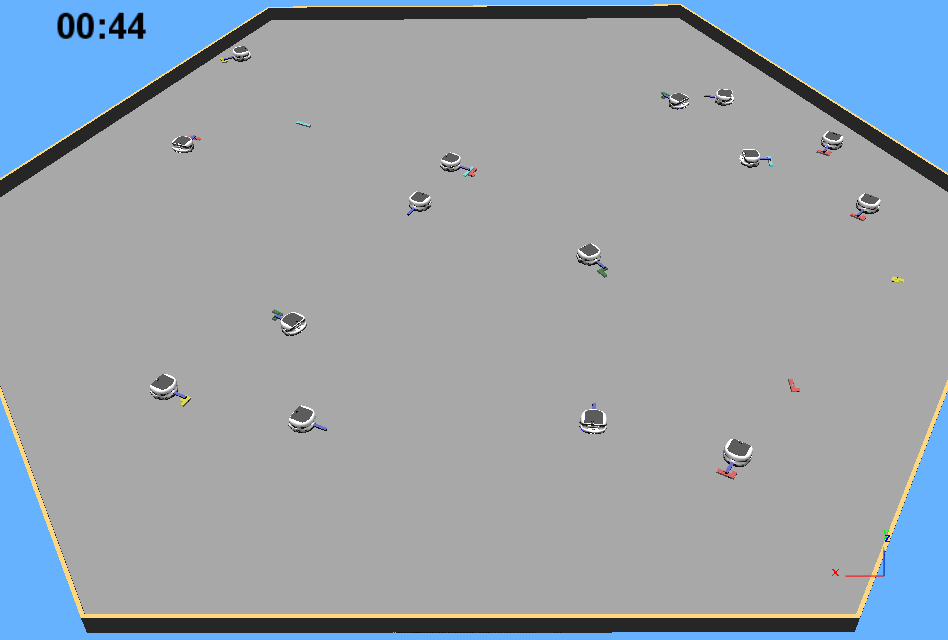
\includegraphics[width=8cm]{img/overall_arena_3.png}
\caption{Snapshot of the arena in the realistic physical simulation.
Robots carry parts at the end of a protruding bar.}
\label{fig:overall_arena}
\end{figure}

% subsection stochastic_assembly (end)

\section{MACRO-CONTINUOUS MODELS}
   \subsection{Definitions}
Interactions between parts and robots in the assembly system are
modeled in the form of a Chemical Reaction Network (CRN).  A set of
reactions can be represented as a directed graph, ${\cal G} = ({\cal
V}, {\cal E})$. The set of vertices, ${\cal V}$, signifies the {\it
complexes}, which are the combinations of parts and/or robots that
appear before and after reaction arrows. The set of directed edges,
${\cal E}$, represents the reaction pathways between the complexes.
Each pathway is denoted by an ordered pair $(i,j) \in {\cal V}
\times {\cal V}$, which means that that complex $i$ transforms into
complex $j$, and is associated with a positive {\it reaction rate
constant}.

Each part of type $i$ in Fig. \ref{fig:assembly_plans} is symbolized
by $X_i$, and a robot is symbolized by $X_R$.  $X_i$ may be further
classified as $X_i^u$, an unclaimed part on the ground, or as
$X_i^c$, a claimed part $i$ and the robot that is carrying it. Let
$M$ be the number of these variables, or {\it species}, in a model
of the system. Then $\mathbf{x}(t) \in \mathbb{R}^M$ is the vector
of the species populations, which are represented as continuous
functions of time $t$.

\subsection{Complete macro-continuous model} % (fold)
\label{sub:complete_macro_continuous_model}

We define a CRN that represents each possible action in the
micro-continuous model of the assembly system:
\begin{eqnarray}
X_R + X_1^u ~~\xrightarrow{e_1} ~~ X_1^c &  & X_R + X_5^u ~~\xrightarrow{e_5} ~~ X_5^c \nonumber \\
X_R + X_2^u ~~\xrightarrow{e_2} ~~ X_2^c &  & X_R + X_6^u ~~\xrightarrow{e_6} ~~ X_6^c \nonumber \\
X_R + X_3^u ~~\xrightarrow{e_3} ~~ X_3^c &  & X_R + X_7^u ~~\xrightarrow{e_7} ~~ X_7^c \nonumber \\
X_R + X_4^u ~~\xrightarrow{e_4} ~~ X_4^c &  & X_R + X_8^u ~~\xrightarrow{e_8} ~~ X_8^c \nonumber \\
X_1^c + X_2^c \xrightarrow{k_1^+} X_5^c + X_R &  &  X_2^c + X_7^c \xrightarrow{k_4^+} X_{F1}^c + X_R \nonumber \\
X_3^c + X_4^c \xrightarrow{k_2^+} X_6^c + X_R & & X_2^c + X_5^c \xrightarrow{k_5^+} X_{8}^c + X_R \nonumber \\
X_5^c + X_6^c \xrightarrow{k_3^+} X_7^c + X_R & & X_6^c + X_8^c \xrightarrow{k_6^+} X_{F2}^c + X_R \nonumber \\
X_5^c \xrightarrow{k_1^-} X_1^c + X_2^u &  &  X_{F1}^c \xrightarrow{k_4^-} X_{7}^c + X_2^u \nonumber \\
X_6^c \xrightarrow{k_2^-} X_3^c + X_4^u & & X_8^c \xrightarrow{k_5^-} X_{5}^c + X_2^u\nonumber \\
X_7^c \xrightarrow{k_3^-} X_6^c + X_5^u & & X_{F2}^c
\xrightarrow{k_6^-} X_{8}^c + X_6^u
\label{eq:complete_macro_continous}
\end{eqnarray}

In this CRN, $e_i$ is the rate at which a robot encounters a part of
type $i$, $k_i^+$ is the rate of assembly process $j$, and $k_i^-$
is the rate of disassembly process $j$.  We theoretically estimate
these rates as functions of the following probabilities:
\begin{equation}
e_i = p^e~, ~~~~k_i^+ = p^e \cdot p^a_i \cdot p_i^+~, ~~~~k_i^- =
p_i^-~. \label{eq:rateDef}
\end{equation}

$p^e$ is the probability that a robot encounters a part or another
robot.  Using the assumption that robots and parts are distributed
uniformly throughout the arena, we calculate $p^e$ from the
geometrical approach that is used to compute probabilities of
molecular collisions~\cite{Gillespie:1992p8126, Correll:2006p8328}:
$p^e~\approx~v T w / A$, where $v$ is the average robot speed, $T$
is a timestep, $A$ is the area of the arena, and $w$ is twice a
robot's communication radius, since this is the range within which a
robot detects a part or robot and initiates an assembly process.

%~\cite{Gillespie:1992p8126, Puchalka:2004p4312, Turner:2004p4446,
%Correll:2007p8184, Correll:2007p8236, Correll:2006p8328}:

%the width of a robot's detection range, which is

$p^a_i$ is the probability of two robots successfully completing
assembly process $i$; it depends on the part geometries.

$p_i^+$ is the probability of two robots starting assembly process
$i$, and $p_i^-$ is the probability per unit time of a robot
performing disassembly process $i$.  These are the {\it tunable
parameters} of the system.

We compute $p^a_i$ and the parameters for $p^e$ using measurements
from the micro-continuous model (Webots simulations): $A = 23.4~
m^2$ (hexagon of radius $3~m$), $w = 1.2~ m$, $v_R = 0.128~m/s$ from
an average over $50$ runs, and $\mathbf{p^a} =
[0.9777~0.9074~0.9636~0.9737~0.8330~1.0]$ (entries follow the
numbering of the associated reactions) from averages over $100$
runs.  We set $T=1 ~s$.

In the thermodynamic limit, which includes the condition that
populations approach infinity, the physical system represented by
\eqref{eq:complete_macro_continous} can be abstracted to an ODE
model \cite{Gillespie:2007p1788}.  This is illustrated in the next
section.  We numerically integrate this macro-continuous model with
the rates we calculated and also use the StochKit
toolbox~\cite{Li:2008p11431} to efficiently perform a stochastic
simulation of the macro-discrete model.  We compare the results to
those for the micro-continuous model in Fig.
\ref{fig:img_complete_model_results}, using $p_i^+=1, ~p_i^-=0 ~~
\forall i$. The results for all models are very similar, although
discrepancies arise from two factors. First, certain events that
happen in the physical simulation are not modeled: parts sticking
together or being wedged against a wall, and deviations from the
assumption of uniform spatial distribution. Second, the ODE
approximation is valid only for large numbers of parts, and the
system modeled had only $15$ robots and $15$ parts. Overall, the
macro-continuous model accurately predicts the evolution of part
populations, and hence we can use it to design the rates to direct
the system's behavior, provided that the system has very large
numbers of parts.

%We can most effectively use it to design the rates to direct the
%system's behavior when the system contains very large numbers of
%parts.

%so our $15$-robot, $15$-part system should be expanded to most
%effectively use the ODE model as a design tool.



%and we used only $15$ robots and $15$ parts.  To most effectively
%use the ODE model as a design tool, the system should contain many
%more parts.


%However, the macro-discrete model is still accurate for even smaller
%populations (results not shown), which validates our

%arise in the physical simulation and prevent some assemblies from
%completing; these effects are not modeled. Second,

%The ODE simulation populations are incorrectly small, as we use only
%15 robots and pieces, where as the ODE approximation is valid only
%for big copy numbers.

%shows that the rates we computed closely capture the system's
%dynamics, and

%is mathematically equivalent to

%, which is based on a Gillespie Stochastic Simulation Algorithm
%\cite{Gillespie:2007p1788},




%We use the complete macro to fit the experimental data
%quantitatively under some reaction rates.

%Toward this end, we reformulate the rates as follows:

%      For chemical process, the probability of collision depends
%          on the volume swept by one molecule, which gives the probability that another
%           molecule will collide it in the next $dt$.

% $p_i^a$ can be easily measured, or assumed to be $1$ if the robots manage
% to align the pieces correctly before each assembly step.


\begin{figure}[t]
\centering
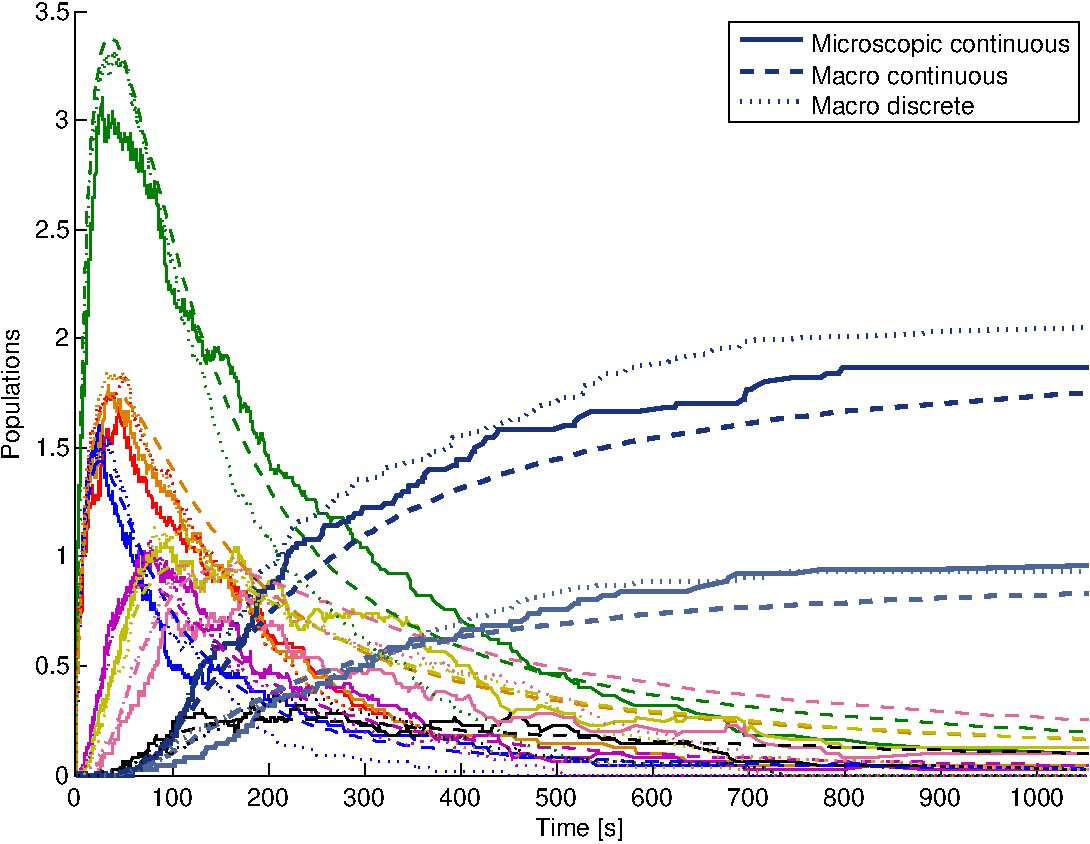
\includegraphics[width=8cm]{img/complete_model_results.pdf}
\caption{Part populations in the complete macro-continuous,
macro-discrete, and micro-continuous models for $3$ final assemblies
and $15$ robots.  Macro-discrete and micro-continuous results are
averaged over 100 runs.} \label{fig:img_complete_model_results}
\end{figure}

\subsection{Reduced macro-continuous model} % (fold)
\label{sub:simple_macro_continuous_model}
    We simplify the complete model by abstracting away robots and retaining
    only interactions between parts, assuming that the time to find a
part is small and there are more robots than parts:
    \begin{eqnarray}
        X_1 + X_2 ~~{\mathop{\rightleftharpoons}_{k_1^-}^{k_1^+}}~~ X_5 & \quad &  X_2 + X_7 ~~{\mathop{\rightleftharpoons}_{k_4^-}^{k_4^+}}~~ X_{F1} \nonumber \\
        X_3 + X_4 ~~{\mathop{\rightleftharpoons}_{k_2^-}^{k_2^+}}~~ X_6 & & X_2 + X_5 ~~{\mathop{\rightleftharpoons}_{k_5^-}^{k_5^+}}~~ X_8 \nonumber \\
        X_5 + X_6 ~~{\mathop{\rightleftharpoons}_{k_3^-}^{k_3^+}}~~ X_7 & & X_6 + X_8 ~~{\mathop{\rightleftharpoons}_{k_6^-}^{k_6^+}}~~ X_{F2}
        \label{eq:reduced_macro_continuous}
    \end{eqnarray}
    The rates are also defined by
    equation~\eqref{eq:rateDef}.

%This model should
%    converge to the same equilibria as the complete
%    model, but its transient regime differs since we removed the
%    delays that arise from robot interactions
%    with free components and other robots.

We define a vector $\mathbf{y(x)} \in \mathbb{R}^{12}$ in which
entry $y_i$ is the part or product of parts in complex $i$:
\begin{eqnarray} \mathbf{y(x)} = && [x_1
x_2~~x_5 ~~x_3 x_4 ~~x_6 ~~x_2 x_7 ~~x_{F1} \nonumber \\  && x_5
x_6~~ x_7~~x_2 x_5 ~~x_8~~ x_6 x_8 ~~x_{F2}]^T~. \label{eq:ydef1}
\end{eqnarray}
We also define a matrix $\mathbf{M} \in \mathbb{R}^{10 \times 12}$
in which each entry $M_{ji}$, $j=1,...,10$, of column $\mathbf{m}_i$
is the coefficient of part type $j$ in complex $i$ ($0$ if absent).
We relabel the rate associated with reaction $(i,j) \in \cal{E}$ as
$k_{ij}$ and define a matrix $\mathbf{K} \in \mathbb{R}^{12 \times
12}$ with entries
\begin{equation}
K_{ij} =  \left\{
\begin{array}{lll}
k_{ji} &\mbox{ if }& i \neq j~, ~~(j,i) \in \mathcal{E}~, \\
0 &\mbox{ if }& i \neq j~, ~~(j,i) \notin \mathcal{E}~,\\
-\sum_{(i,l)\in {\mathcal E}} k_{il} &\mbox{ if }& i=j~.
\end{array} \right. \label{eq:Kdef}
\end{equation}
Then our ODE abstraction of the system can be written in the
following form \cite{Chaves:2004p11839}:
\begin{equation}
\mathbf{\dot{x}} = \mathbf{M}\mathbf{K}\mathbf{y}(\mathbf{x})~.
\label{eq:matrixODE}
\end{equation}

%$K_{ij} = k_{ji}$ if $i \neq j~, (j,i) \in \mathcal{E}$; $0$ if $i
%\neq j~, (j,i) \notin \mathcal{E}$; and $-\sum_{(i,l)\in {\mathcal
%E}} k_{il}$ if $i=j$.

One set of linearly independent conservation constraints on the part
quantities is:
\begin{equation}
%\left\lbrace
\begin{array}{lll}
x_3 - x_4 &=& N_1 \\
x_1+x_5+x_7+x_8+x_{F1}+x_{F2} &=& N_2 \\
x_2+x_5+x_7+2(x_8+x_{F1}+x_{F2}) &=& N_3 \\
x_3+x_6+x_7+x_{F1}+x_{F2} &=& N_4
\end{array}
%\right.
\label{eq:cons}
\end{equation}
where $N_i$, $i=1,...,4$, are computed from the initial part
quantities.

%This simplification allows us to study the stability of this system:

\begin{theorem}\label{thm:unique_equilibrium}
System \eqref{eq:matrixODE} subject to \eqref{eq:cons} has a unique,
stable equilibrium $\mathbf{\bar{x}} > \mathbf{0}$.
\end{theorem}
\begin{proof}  Each equilibrium of the system, $\{\mathbf{\bar{x}}
~|~\mathbf{M}\mathbf{K}\mathbf{y(\bar{x})} = \mathbf{0}\}$, can be
classified as either a {\it positive} equilibrium $\mathbf{\bar{x}}
> \mathbf{0}$ or a {\it boundary} equilibrium in which $\bar{x}_i
= 0$ for some $i$, which can be found by solving
$\mathbf{y(\mathbf{\bar{x}})} =
\mathbf{0}$~\cite{Chaves:2004p11839}.  From definition
\eqref{eq:ydef1} of $\mathbf{y(x)}$, it can be concluded that in
each boundary equilibrium, all $x_i = 0$ except for one of the four
combinations of variables $(x_1,x_3), (x_1,x_4), (x_2,x_3),
(x_2,x_4)$.  Since we only consider systems that can produce
$x_{F1}$ and $x_{F2}$, it is not possible for the system to reach
any of these equilibria; each one lacks two part types needed for
the final assemblies.

%whose rows are each obtained by subtracting a column of $\mathbf{M}$
%associated with a reactant in a particular reaction from a column
%associated with a product

The {\it deficiency} $\delta$ of a reaction network is the number of
complexes minus the number of linkage classes, each of which is a
set of complexes connected by reactions, minus the network rank,
which is the rank of the matrix with rows $\mathbf{m}_i -
\mathbf{m}_j$, $(i,j) \in \cal{E}$ \cite{Feinberg:1995p9419}.
 Network \eqref{eq:reduced_macro_continuous} has $12$ complexes, $6$
linkage classes, and rank $6$; hence, $\delta = 0$.  Also, the
network is {\it weakly reversible} because whenever there is a
directed arrow pathway from complex $i$ to complex $j$, there is one
from $j$ to $i$.  Because the network has deficiency $0$, is weakly
reversible, and does not admit any boundary equilibria, it has a
unique, globally asymptotically stable positive equilibrium
according to Theorem 4.1 of \cite{Siegel:2000}.
\end{proof}

%These properties, along with the fact that the system kinetics are
%mass-action, satisfy the criteria for applying the Deficiency Zero
%Theorem \cite{Feinberg:1995p9419}, which gives the result that the
%system has exactly one positive steady state, which is
%asymptotically stable.  In fact, by Theorem 4.1 of
%\cite{Siegel:2000}

%\cite{Feinberg:1987p9428}

% subsection simple_macro_continuous_model (end)

\section{RATE OPTIMIZATION}\label{sec:optimization}
   We consider the problem of designing the system described by model
\eqref{eq:matrixODE} subject to \eqref{eq:cons} to produce desired
quantities of parts as quickly as possible. The objective will be
posed as the design of {\it optimal rates} $k_i^+, k_i^-$,
$i=1,...,6$, which define an {\it optimal rate matrix}
$\mathbf{K}^*$ according to \eqref{eq:Kdef}, that minimize the
convergence time of the system to a vector of target part
quantities, $\mathbf{x^d}$. Note that although only the amounts of
the final assemblies $F1$ and $F2$ may need to be specified in
practice, our optimization problem requires that target quantities
of {\it all} parts be defined.

We first specify $x_1^d, x_2^d, x_3^d, x_5^d, x_8^d$ and a parameter
\begin{equation}
\alpha \equiv x_{F1}^d/(x_{F1}^d+x_{F2}^d)~. \label{eq:alpha}
\end{equation}
Then we compute the dependent variables $x_4^d, x_6^d, x_7^d,$ and
$x_{F1}^d+x_{F2}^d$ from the conservation equations \eqref{eq:cons}
and definition \eqref{eq:alpha} and check that they are positive to
ensure a valid $\mathbf{x^d}$. In this way, we can keep
$x_{F1}^d+x_{F2}^d$ and the target non-final part quantities
constant while adjusting the ratio between $x_{F1}$ and $x_{F2}$
using $\alpha$.  Theorem \ref{thm:unique_equilibrium} shows that we
can achieve $\mathbf{x^d}$ from any initial distribution
$\mathbf{x^0}$ by specifying that $\mathbf{\bar{x}} = \mathbf{x^d}$
through the following constraint on $\mathbf{K}$,
\begin{equation}
\mathbf{M}\mathbf{K}\mathbf{y(x^d)} = \mathbf{0}~.
\label{eq:equilConstr}
\end{equation}

%The rates $k_i^+, k_i^-$ can be chosen so that the assembly system
%yields a target piece distribution $\mathbf{x^d} > \mathbf{0}$
%starting from {\it any} initial distribution of pieces.

%, as will be discussed later in this section.

%We can define measures of this time by reformulating the system in
%terms of new variables.

Now we consider the aspect of minimizing the convergence time to
$\mathbf{x^d}$.  We quantify this time in terms of the system {\it
relaxation times} $\tau_i$, $i=1,...,6$, the times in which
different modes (dynamically independent variables) of the the
system converge to a stable equilibrium after
perturbation~\cite{bib:Heinrich1977,bib:Jamshidi2008}.  Various
measures of the average relaxation time of a CRN have been defined,
but they are applicable only under certain conditions, such as a
linear reaction sequence \cite{bib:Heinrich1991}.  For instance, one
such measure was minimized in the optimization of rates for the
linear chain in \cite{Schuster:1987p11838}.

To estimate the relaxation times, we first reformulate the system in
terms of new variables.  Define $v_i$, $i=1,...,6$, as the
difference between the forward and reverse fluxes associated with
reaction $i$ in system \eqref{eq:reduced_macro_continuous}. For
example, $v_1 = k_1 x_1 x_2 - k_2 x_5$.  Let $\mathbf{v(x)} =
[v_1~...~v_{6}]^T$ and let $\mathbf{S} \in \mathbb{R}^{6 \times 10}$
denote the stoichiometric matrix of the system, which is defined
such that model \eqref{eq:matrixODE} can be written as
\cite{bib:Heinrich1996}:
\begin{equation}
\mathbf{\dot{x}} = \mathbf{S} \mathbf{v(x)}~.
\end{equation}
        %The entries $s_{ij}$ of $\mathbf{S}$ for this model are $-1$, $0$,
        %or $1$.

%Our assembly system is similar to a model of a biochemical network
%with mass action kinetics.

%we take a common approach in studying the dynamical properties of a
%CRN,

The dynamical properties of a CRN are often analyzed by linearizing
the ODE model of the system about an equilibrium and studying the
properties of the associated Jacobian matrix $\mathbf{J} =
\mathbf{S} \mathbf{G}$, where the entries of $\mathbf{G}$ are
$G_{ij} = dv_i/dx_j$ \cite{bib:Jamshidi2008}.  Denoting the
eigenvalues of $\mathbf{J}$ by $\lambda_i$, a common measure of
relaxation time is $\tau_i = 1/|Re(\lambda_i)|$.  Since the
$\lambda_i$ are negative at a stable equilibrium, one way to yield
fast convergence is to choose rates
 that minimize the largest $\lambda_i$. However,
in our system it is very difficult to find analytical expressions
for the $\lambda_i$.  We use an alternative estimate of relaxation
time that is also derived by linearizing the system around its
equilibrium $\mathbf{x^d}$ \cite{bib:Heinrich1996},
\begin{equation}
\tau_j = \left( \sum_{i=1}^{10} (-s_{ij}) \frac{d v_j}{d x_i}
\right)^{-1}_{\mathbf{x} = \mathbf{x^d}} ~.\label{eq:tau}
\end{equation}


%we explore other ways of quantifying convergence time.

%, as was done for a linear chain of enzymatic reactions
%in~\cite{Schuster:1987p11838}

%We use a general estimate of the relaxation time for each reaction


Each reaction $j$ in system \eqref{eq:reduced_macro_continuous} is
of the form $X_k + X_l
~~{\mathop{\rightleftharpoons}_{k_j^-}^{k_j^+}}~~ X_m$.  Thus, $v_j
= k_j^+ x_k x_l - k_j^- x_m$, and the entries of column $j$ in
$\mathbf{S}$ are all $0$ except for $s_{kj} = s_{lj} = -1$ and
$s_{mj} = 1$.  Then according to equation \eqref{eq:tau}, the
relaxation time for each reaction is
\begin{equation}
\tau_j = (k_j^+(x_k^d + x_l^d) + k_j^-)^{-1}~. \label{eq:tauSys}
\end{equation}

Define $\mathbf{k} \in \mathbb{R}^{12}$ as the vector of all rates
$k_i^+, k_i^-$. Using equation \eqref{eq:tauSys}, we define two
possible objective functions $f:\mathbb{R}^{12} \rightarrow
\mathbb{R}$, the average $\tau_j^{-1}$ and the minimum
$\tau_j^{-1}$, to {\it maximize} in order to produce fast
convergence to $\mathbf{x^d}$:
\begin{eqnarray}
f_{ave}(\mathbf{k}) &=& \tfrac{1}{6} \sum_{j=1}^{6} \tau_j^{-1}~, \label{eq:obj1} \\
f_{min}(\mathbf{k}) &=& \min \{ \tau_1^{-1}, \ldots,
\tau_{6}^{-1}\}~. \label{eq:obj2}
\end{eqnarray}

%The first is the average inverse relaxation time,
%The second is the minimum inverse relaxation time,

Finally, we write the rates $k_i^+, k_i^-$ in terms of the tunable
probabilities $p_i^+, p_i^-$ using equation \eqref{eq:rateDef} and
define these probabilities as the optimization variables.  Let
$\mathbf{p} \in \mathbb{R}^{12}$ be the vector of all $p_i^+,
p_i^-$.  Then the optimization problem can be posed as
\textbf{Problem P} below.  It will be referred to as \textbf{Problem
P1} when $f = f_{ave}$ and as \textbf{Problem P2} when $f =
f_{min}$.

\vspace{3mm} \noindent \textbf{[P] } \hspace{2mm} ~maximize ~~
$f(\mathbf{k(p)})$

\vspace{1mm}

\hspace{7mm} subject to ~~$\mathbf{M}\mathbf{K(p)}\mathbf{y(x^d)} =
\mathbf{0}$, ~~$\mathbf{0} \leq \mathbf{p} \leq \mathbf{1}$~.
\vspace{2mm}

Problems P1 and P2 are both linear programs, which can be solved
efficiently.  To check that they do in fact minimize convergence
time, we implemented a Monte Carlo method \cite{ref:Landau00}, which
is more computationally expensive, to find the $\mathbf{k(p)}$ that
directly minimizes this time. We measure the degree of convergence
to $\mathbf{x^d}$ by $\Delta(\mathbf{x}) =
||\mathbf{y(x)}-\mathbf{y(x^d)}||_2$ and say that one system
converges faster than another if it takes less time for
$\Delta(\mathbf{x})$ to decrease to some small fraction, here
defined as $0.1$, of its initial value.  At each iteration,
$\mathbf{k(p)}$ is perturbed by a random vector and projected onto
the null space of linearly independent rows of a matrix $\mathbf{N}$
defined such that $\mathbf{N}\mathbf{k} =
\mathbf{M}\mathbf{K}\mathbf{y(x^d)} = \mathbf{0}$.  Once
$\mathbf{k(p)}$ also satisfies $\mathbf{0} \leq \mathbf{p} \leq
\mathbf{1}$, it is used to simulate the reduced macro-continuous ODE
model to find $\Delta(\mathbf{x})$ after some time. Since the system
is stable by Theorem \ref{thm:unique_equilibrium},
$\Delta(\mathbf{x})$ always decreases monotonically with time, so a
Newton scheme can be used to compute the exact time $t_{0.1}$ when
$\Delta(\mathbf{x}) = 0.1\Delta(\mathbf{x^0})$.

%, its $k_i^+$ entries are scaled by $p_i^e p_i^a$,

%adjustable parameters of the physical assembly system.   Each
%forward rate $k_j^+$ is defined by the product in equation
%\eqref{eq:reaction_assembly_rate} multiplied by a probability of
%starting the assembly, $p_j^+ \in \{0, 1\}$.

%Since this problem can be formulated as the
%minimization of a linear combination of the entries of $\mathbf{p}$
%subject to a set of linear equality and inequality constraints on
%$\mathbf{p}$, it is a linear program, which can be solved
%efficiently.

        % subsubsection convex_program_definition (end)

    % subsection design_of_optimal_rates (end)

 %   \subsection{Optimization implementation} % (fold)
  %  \label{sub:optimization_implementation}
 %       In order to optimize the convex programs P1 and P2, we use a framework for Matlab, YALMIP\cite{Lofberg:2004p11461}. It allows us to define our optimization variables, objective function and constraints and to apply a semidefinite programming solving algorithm, running in polynomial time \cite{Lofberg:2004p11461}.
    % subsection optimization_implementation (end)
% section methodology (end)

%$p_j^e$ is the encountering probability defined by \eqref{eq:encountering_probability},
%dependent on some parameters and $p_j^a$ is the assembly success rate,
%which we measure as explained in Section~\ref{ssub:stochastic_constant_rates_values}.

\section{RESULTS}
	\subsection{Optimization of rates} % (fold)
\label{sub:optimization_of_rates}

    We solved optimization problems P1 and P2 for $\alpha \in \{0.01, 0.02, \ldots, 0.99\}$
    using $\mathbf{x^0} = [60~120~60~60~\mathbf{0}]^T$ and $\mathbf{x^d} =
    [0.5~2.5~1~1~0.5~1~1~1~57\alpha~57(1-\alpha)]^T$.  As Table I shows,
    the computed rates are constant for each $\alpha$ except for
    those corresponding to assembly and disassembly processes $4$ and $6$.
    This means that the system is flexible enough to yield any $\alpha$
    when only the rates of assembling and breaking apart the final
    assemblies are modified.  We also ran the Monte Carlo program
    for $\alpha=0.4$.  For the optimal set of rates, which were very similar to those for
    Problem P1, $t_{0.1} = 4.69$, as compared to $4.68$ for Problem P1 and $8.49$ for P2.  This
    provides evidence that Problem P1 is minimizing the system convergence time.



    \begin{table*}[t!]
        \begin{center}
        \caption{Values of optimized rates for varying $\alpha$. \textit{Continuous} rates
        evolve continuously with respect to $\alpha$.}
        \begin{tabular}{|c|c|c|c|c|c|c|}
            \hline
            \textbf{Reaction} $\mathbf{i}$ & \textbf{1} & \textbf{2} & \textbf{3} & \textbf{4} & \textbf{5} & \textbf{6} \\
            \hline
            \textbf{P1 Optimized} $\mathbf{p^+_i}$ & \multicolumn{6}{c|}{1.0} \\
            \hline
            \textbf{P1 Optimized} $\mathbf{p^-_i}$ & 0.01885 & 0.00754 & 0.00377 & \textit{continuous} & 0.00942 & \textit{continuous}\\
            \hline
            \textbf{P2 Optimized} $\mathbf{p^+_i}$ & 0.36 & 0.666 & 1.0 & \textit{continuous} & 0.4705 & \textit{continuous}\\
            \hline
            \textbf{P2 Optimized} $\mathbf{p^-_i}$ & 0.006855 & 0.005027 & 0.00377 & \textit{continuous} &  0.00443 & \textit{continuous} \\
            \hline
        \end{tabular}
        \end{center}
        \label{tab:optimized_rates}
    \end{table*}

     % ($k_4^-=0.0008269$, $k_6^-=0.0002205$)

%To verify the effect of the optimization on the system convergence,

We integrated the reduced macro-continuous model for $\alpha=0.4$
and $\alpha=0.8$ using the optimized rates from Problems P1 and P2
and a set of non-optimal rates that were chosen to satisfy
constraint \eqref{eq:equilConstr} and $\mathbf{0} \leq \mathbf{p}
\leq \mathbf{1}$ but were not optimized for some objective.  The
evolution of the model for each set of rates is shown in
Fig.~\ref{fig:ODEalpha_pt4}, with time in log-scale.  The optimized
systems first quickly converge to an ``intrinsic equilibrium" at $t
\approx 10^2$ that is independent of $\alpha$ and then redistribute
much more slowly to the target ratios, which are attained for all
set of rates.  For both $\alpha$, the optimized models converge
faster to equilibrium than the non-optimal model. For $\alpha=0.4$,
the non-optimal model displays a large over- and under-shooting of
the target ratios, whereas the optimized models converge quickly
with little or none of this effect.  Problem P2 produces a more
efficient system in this respect, although both optimized models
converge at comparable rates.

%Since the optimized models converge to the target ratio at
%comparable rates, \eqref{eq:obj1} and \eqref{eq:obj2} are both good
%objective functions

%Both objective functions used in Problems P1 and P2 seem good
%heuristics with respect to convergence time. Both have comparable
%performances, so we cannot decide between the two objectively.

%For $\alpha=0.4$, the non-optimal set of rates undergoes a flipping
%of ratios at $t=10^5$.


    \begin{figure}[!t]
        \centering
        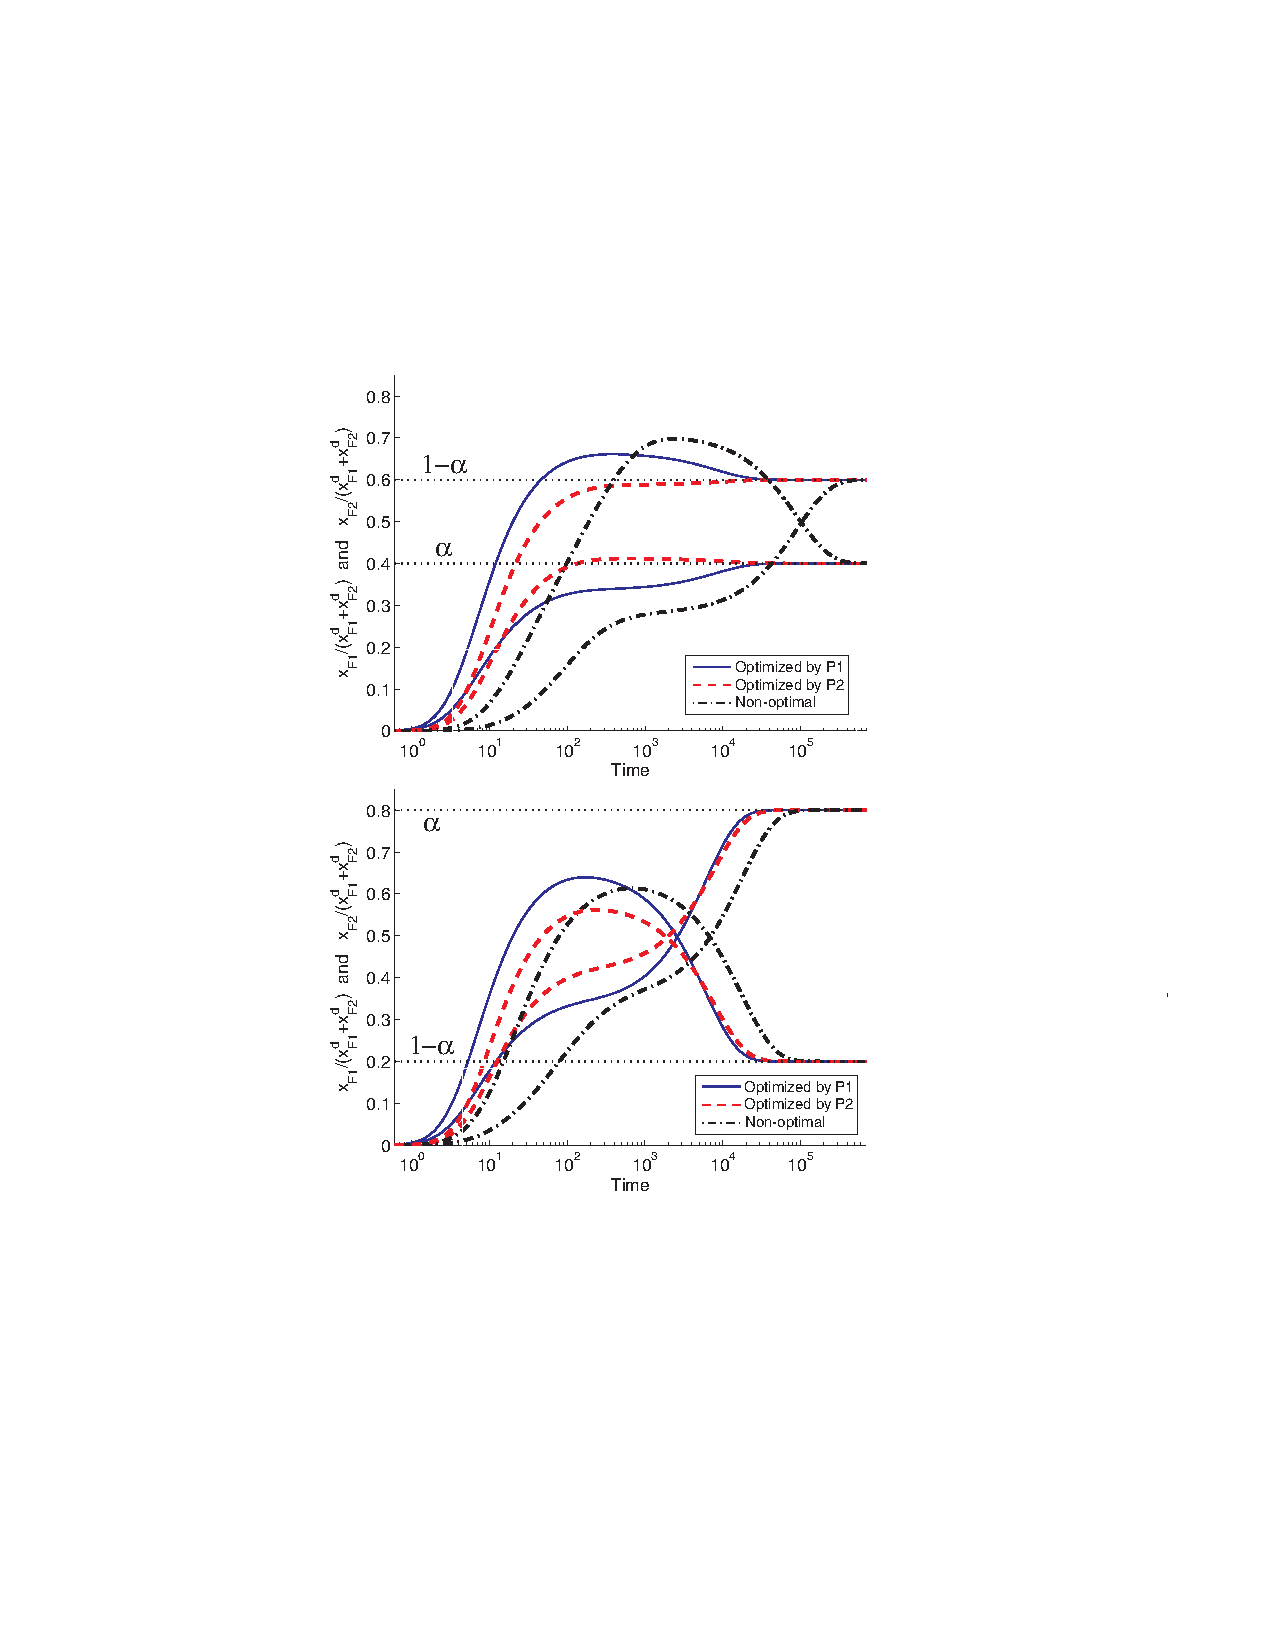
\includegraphics[trim= 40mm 75mm 10mm 60mm, clip,scale=0.65,angle=0]{img/ODE_alpha_comp2.pdf}
                %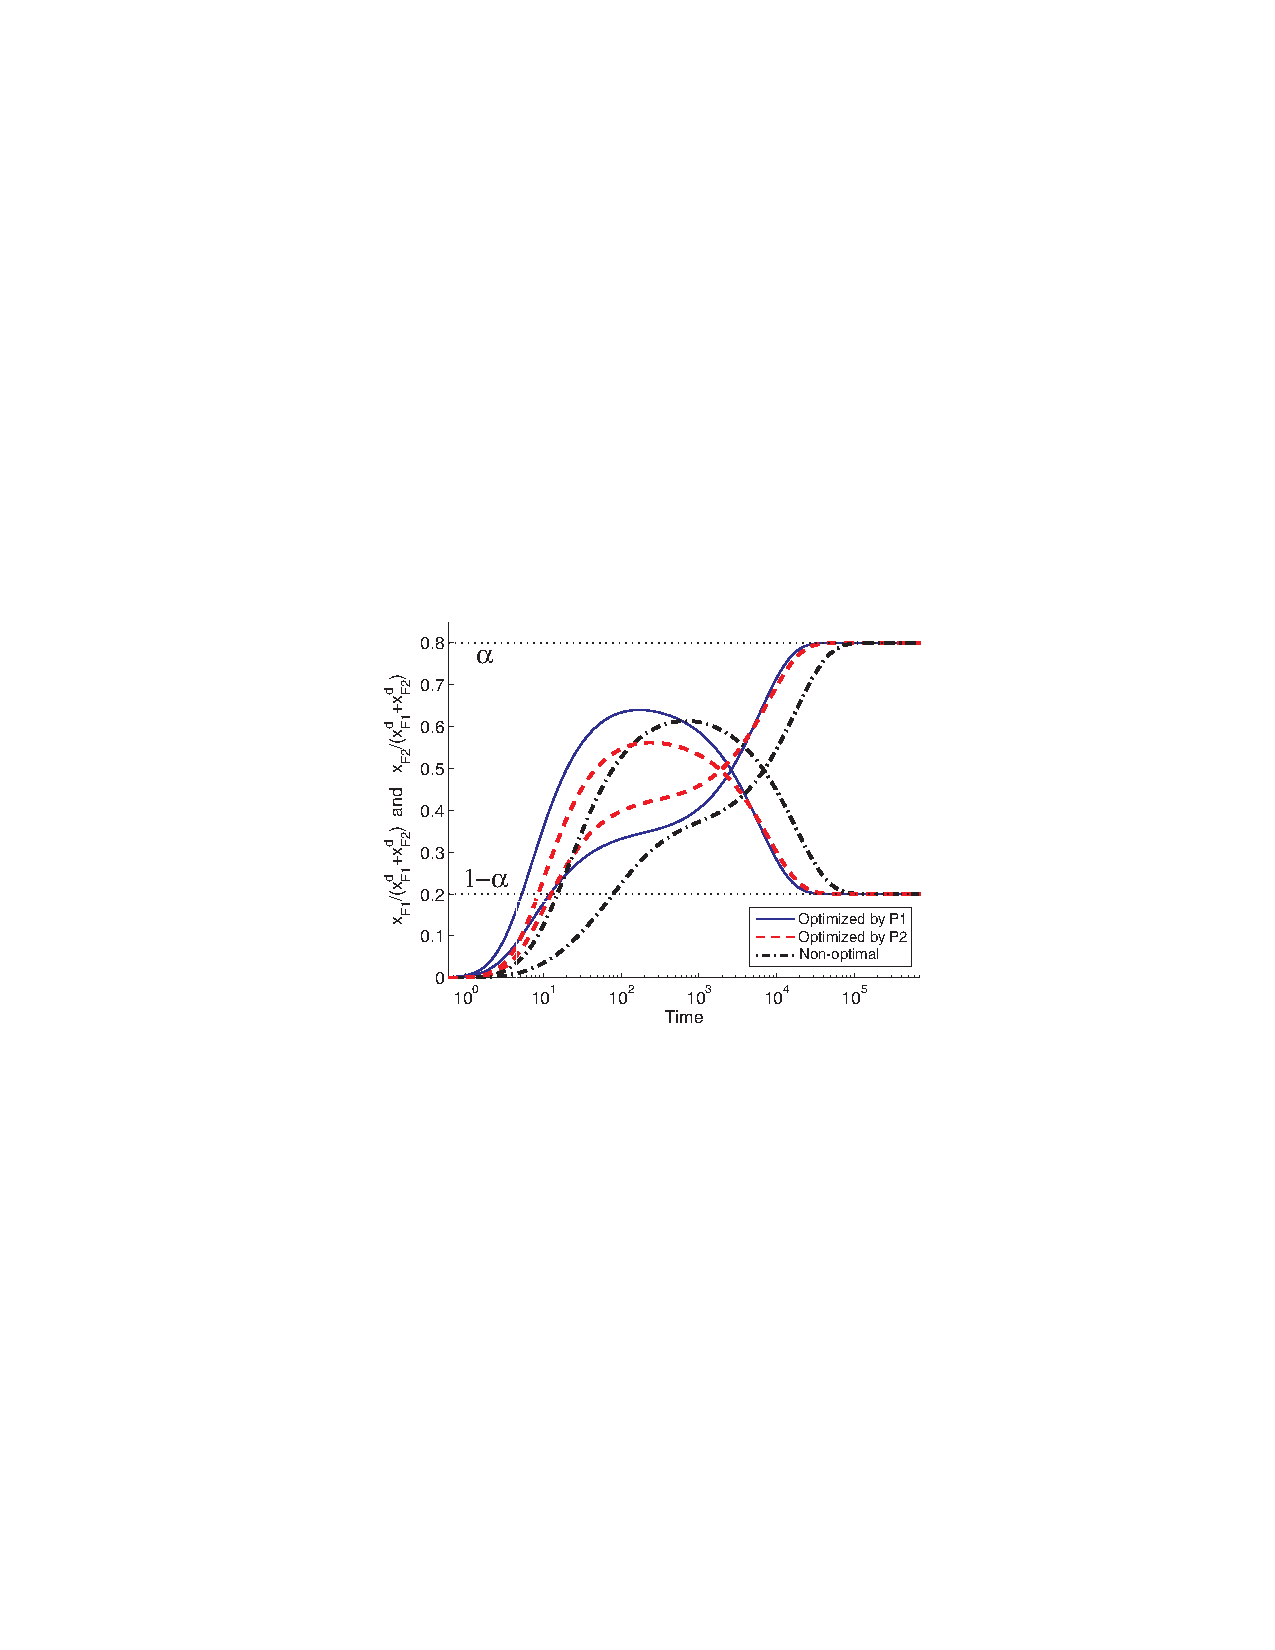
\includegraphics[trim= 70mm 85mm 70mm 85mm, clip,scale=0.7,angle=0]{img/ODE_alpha_comp_apt8.pdf}
        \caption{Evolution of final assembly ratios in the reduced macro-continuous model
         for $\alpha=0.4$ (top) and $\alpha = 0.8$ (bottom), using rates optimized by
         Problems P1 and P2 and non-optimal rates.}
        \label{fig:ODEalpha_pt4}
    \end{figure}


% subsection optimization_of_rates (end)

\subsection{Mapping rates onto the micro-continuous model} % (fold)
\label{sub:mapping_on_the_microscopic_model}

For $\alpha=0.4$, we mapped the rates optimized by Problem P1 and
the non-optimal rates onto the micro-continuous model to see whether
the physical system would behave similarly to the reduced continuous
model.  We did this in the following way.  Let $R$ be a uniformly
distributed random number between $0$ and $1$ and let $\Delta t$ be
the simulation timestep.  A robot carrying a part that can be
disassembled according to process $i$ computes $R$ at each timestep
and disassembles the part if $R < p_i^- \Delta t$. A robot about to
begin assembly process $i$ computes $R$ and executes the assembly if
$R < p_i^+ \Delta t$.  Fig.~\ref{fig:img_webots_results_alpha04}
shows the time evolution of the micro-continuous model averaged over
$30$ runs for both sets of rates, using $15$ robots and $15$ parts
($3$ final assemblies).  The non-optimal model converges to the
target ratios but initially over- and under-shoots $x_{F1}^d$ and
$x_{F2}^d$, respectively, as in Fig.~\ref{fig:ODEalpha_pt4}.  The
ratios in the optimized model rise quickly to the target ratios but
then deviate from them toward $0.5$.

%- I wanted to say that the convergence to the equilibrium is less
%stable. Actually the convergence is pretty bad if you look at it,
%but  I want to say that this is most likely because of variation
%around the  target ratios.

The discrepancy between the optimized model results and the target
ratios can be explained by inaccurate modeling of some low-level
effects.  In the micro-continuous model, when a robot disassembles a
part, a nearby robot is likely to pick up the fallen component and
quickly reassemble the original part with the other robot, which
generally hasn't traveled far.  This increases the rate of assembly
of the part and violates the well-mixed assumption.  In addition,
robots that pick up dropped parts spend a significant amount of time
carrying them before reassembly, a factor that was abstracted away
in the reduced model.  Adding more robots tends to alleviate this
effect.  Random failures at disassembly, incorrect internal state
definitions by the robots and parts, and collision errors by the
physics engine sometimes occur in the simulation but are not
modeled. Finally, the continuous abstraction may not accurately
capture the system behavior for such a low number of parts. However,
it becomes more computationally expensive to simulate the system as
the number of parts and robots increase.

%simulation speed decreases as the number of parts and robots
%increase.

%means that the number of final assemblies is small compared to the
%nonzero numbers of intermediate assemblies



    \begin{figure}[t]
        \centering
            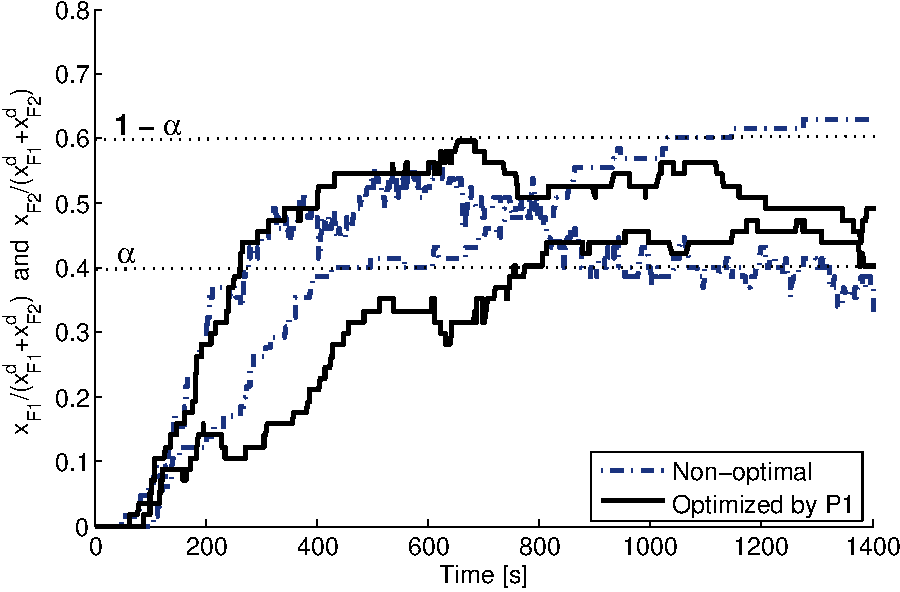
\includegraphics[width=8cm]{img/webots_results_alpha04.pdf}
        \caption{Evolution of final assembly ratios in the micro-continuous model
        for $\alpha=0.4$, using rates optimized by
         Problem P1 and non-optimal rates.}
        \label{fig:img_webots_results_alpha04}
    \end{figure}

% subsection mapping_on_the_microscopic_model (end)


\subsection{Reconfigurable manufacturing} % (fold)
\label{sub:green_manufacturing}

We apply our methodology to a ``green manufacturing" task, in which
finished products are recycled into new products in ratios that
depend on the current demand.  We perform a simulation of the
reduced macro-continuous model that corresponds to a situation in
which robots switch between sets of optimized rates at discrete
points in time to produce different target numbers of parts.  The
sequence of target $\alpha$ is $0.4, 0.99, 0.01$, and $0.5$, and
$\mathbf{x^0}$ is the same as in Section
\ref{sub:optimization_of_rates}.  The system evolution is shown in
Fig.~\ref{fig:img_optim_online_adaptation} using rates from Problem
P1.  The system quickly adapts to new target ratios, although some
take longer to attain than others (e.g. $\alpha=0.5$).  The results
demonstrate that high-level control of the system is possible in
real-time.

    %This high-order goal is directly realizable by changing abruptly the set of
    %reaction rates used by the robots.

    \begin{figure}[t]
        \centering
            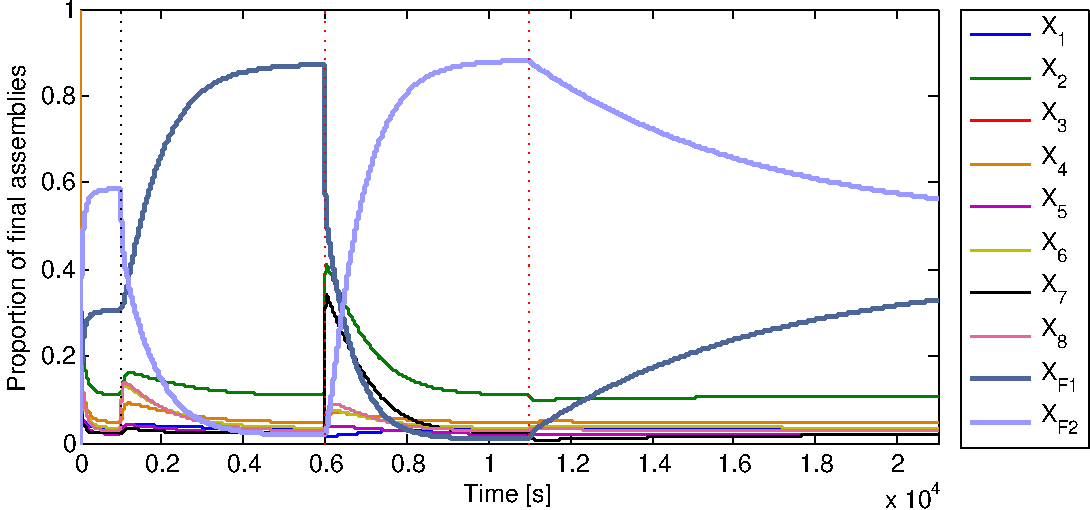
\includegraphics[width=8.5cm]{img/optim_online_adaptation.pdf}
        \caption{Online adaptation of the reduced macro-continuous model to changes in target equilibrium,
        which occur at the vertical dashed lines.}
        \label{fig:img_optim_online_adaptation}
    \end{figure}

% subsection green_manufacturing (end)

%\subsection{Comparison with Deterministic Approach}

\section{DISCUSSION AND FUTURE WORK}
We developed and presented a method to systematically derive
decentralized control policies for a swarm of robots performing
assembly tasks to manufacture different products in response to
varying demand. We represent the system using a multi-level modeling
methodology. The micro-continuous model is derived from the dynamics
of the robots and the assembly task and is implemented on a
physics-based simulator.  The collective behavior of the system,
including the physical interactions between robots, is abstracted to
a macro-continuous ODE model. The model incorporates parameters that
govern the stochastic control policies running on individual robots
for performing the assembly task. By tuning the parameters of the
ODE, we can also tune the performance of the assembly system. This
optimization relies on global stability properties of a specific
class of chemical reaction networks that are modeled by the
macro-continuous model. We implement the optimization as a linear
program with constraints on target amounts of parts at equilibrium,
using two possible objective functions that are based on an estimate
of the system convergence time.  We simulate the macro-continuous
model and observe that it achieves the target final product amounts
faster with optimized rates than with non-optimal rates, and that it
can quickly respond to changes in the target equilibrium.  Finally,
we map the rates onto probabilities of assembly and disassembly in
the micro-continuous model.  We find that the resulting system can
produce the target product amounts, although discrepancies arise due
to violation of the well-mixed property, low part numbers, and
failure to capture certain physical effects in the macro-continuous
model.

Our future work will focus on tuning the macro-continuous model to
match the physical system more closely, addressing in particular the
lack of spatial homogeneity due to a small number of robots and
parts. In addition, we also want to investigate the synthesis of the
discrete assembly plans and incorporate feedback into the process.
This direction draws inspiration from bio-molecular pathways in
which intermediate subassemblies or molecules can promote or inhibit
chemical reactions. We would like to be able to optimize the
discrete assembly plan by constructing feedback loops to improve the
yield rate.


- Optimizing the plan using an expanded model

\bibliographystyle{IEEEtran}
\bibliography{icra09}

\end{document}

